\documentclass[letterpaper,oneside,12pt]{article}
%\documentclass[letterpaper,oneside,12pt]{report}
\usepackage{graphicx}
\usepackage{rotating}
\usepackage[american]{babel}

\selectlanguage{american}

% page layout
%  \setlength{\hoffset}{-1in} 
  %\setlength{\voffset}{-1in}
%  \setlength{\textwidth}{15cm}
%  \setlength{\oddsidemargin}{3.5cm}
%  \setlength{\evensidemargin}{0.2cm}
%  %\setlength{\topmargin}{2.5cm}
%  \setlength{\headsep}{5ex}
%  \setlength{\textheight}{22cm}
%  \renewcommand{\baselinestretch}{1.05}
%  \raggedbottom
%  \newlength{\pictheight}
%  \setlength{\pictheight}{\textheight}
%  \addtolength{\pictheight}{-2cm}

% document
\begin{document}

%\begin{titlepage}
\hspace{-7mm}
\begin{minipage}{\textwidth}
\begin{center}
\vspace{.5cm}
{\huge \bf Software Design Document\\[1.5ex]}
{\large \bf for a specific implementation of `BCI2000'}
\\[1.5cm]
{\Large Gerwin Schalk\\}
{\Large Thilo Hinterberger\\}
{\Large Dennis J. McFarland\\[1.5cm]}
%
\begin{minipage}{13cm}
  \begin{minipage}[c]{13cm}
    \begin{center}
      {\Large \bf New York State Department of Health\\[2ex]}
      {\large \bf Wadsworth Center\\[0.5ex]
       Laboratory of Nervous Systems Disorders\\[4ex]}
      {\Large \bf Eberhard--Karls--Universit\"at T\"ubingen\\[2ex]}
      {\large \bf Medizinische Fakult\"at\\[0.5ex]
       Institut f\"ur Medizinische Psychologie\\[0.5ex]}
    \end{center}
  \end{minipage}
  \\[1.0cm]
  \begin{minipage}[c]{6cm}
    \centerline{
\includegraphics{figures/DOHlogo}}
  \end{minipage}
  \hspace{1.5cm}
  \begin{minipage}[c]{3cm}
    \centerline{
\includegraphics{figures/EKUlogo}}
  \end{minipage}
\end{minipage}
%
\\[0.5cm]
\textbf{Sponsors} \\
\textit{Jonathan R. Wolpaw and Niels Birbaumer}
\\[1.0cm]
{Albany, NY} \\[1ex]
{February 2000--May 2001}
\\[1ex]Updated May 2003, J\"urgen Mellinger
\end{center}
\end{minipage}
\end{titlepage}

\title{D3BOX Task for BCI2000}
%\author{Jennia Hizver, J\"{u}rgen Mellinger, Gerwin Schalk}
\author{Jennia Hizver, Gerwin Schalk}
\maketitle

\newpage
\tableofcontents

\newpage 

\begin{abstract}

The primary purpose of this task is the replication of the 2D center-out task 
(i.e., D2BOX) in a 3D environment. Users can control a cursor towards targets 
using control in two dimensions. Another purpose of this task is the creation of 
generic functions that will allow the creation of any task in a simple 3D 
environment with certain characteristics.

\end{abstract}

\newpage
\section{Functionality}


\newpage
\section{The Environment}

\begin{figure}[ht]
 \centerline{\scalebox{1}{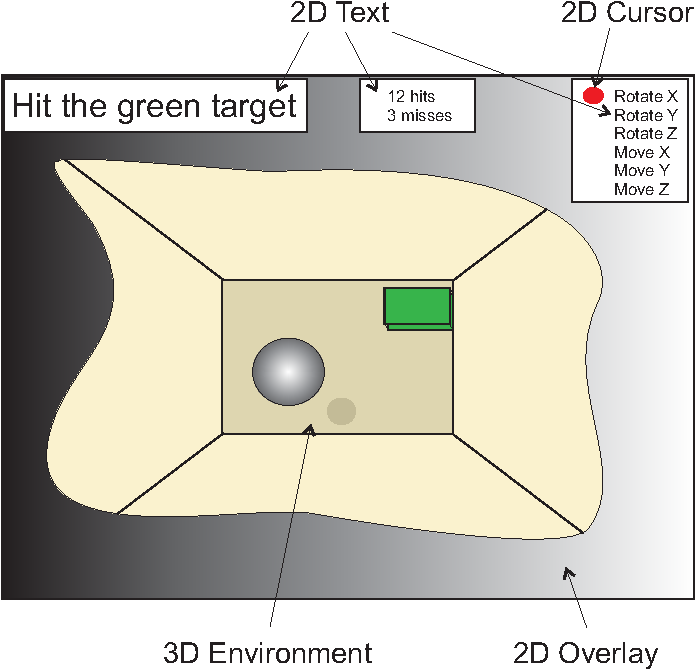
\includegraphics{figure/environment.pdf}}}
 \caption{Graphical Environment.}
 \label{fig:environment}
\end{figure}

\subsection{Rendering}



\subsection{The 3D Environment}

\subsubsection{Predefined Graphic Primitives}
The 3D environment supports any number of predefined graphic primitives. 
Each graphic primitive can be assigned a number of different properties. 
These are:
\begin{itemize}
 \item Element ID
 \item Primitive ID
 \item Primitive-specific properties
 \item Generic properties
       \begin{itemize}
        \item Brightness (0-255)
        \item Transparency (0-255)
        \item Color (RGB)
        \item Texture
       \end{itemize}
\end{itemize}
Supported primitives are spheres (i.e., primitive ID 1), cuboids (i.e., primitive ID 2), 
and infinite planes (i.e., primitive ID 3). The position
of a sphere is defined by midpoint (XYZ) and radius. Textures are mapped using
circular mapping using arbitrary alignment. The position of a cuboid is defined
by a midpoint (XYZ) and a width, height, and depth (to define the extend in 
X, Y, and Z, respectively). Texture mapping is defined by the orientation and
size of a texture. The only supported mapping type is parallel mapping.
Infinite planes are defined by three points in XYZ coordinates. The only supported
texture mapping type is parallel mapping with the texture being parallel to the plane.

Once created, there are certain functions that can be applied to any element.
\begin{itemize}
 \item Change properties
 \item Turn on/off
 \item Move midpoint to XYZ
 \item Test for collision with another element
 \item Rotate element with rotation defined by
       \begin{itemize}
        \item Angles in X, Y, Z
        \item Reference point in X, Y, Z
       \end{itemize}
\end{itemize}


\subsubsection{Custom Graphic Primitives}

In addition to built-in primitives, the system also supports custom graphic 
primitives. These primitives can be defined by loading their 3D structure from a 
file and they support the same methods as the predefined primitives except 
collision detection.


\subsubsection{3D Text}

The system supports any number of 3D text elements. Each text element
is defined by
\begin{itemize}
 \item Font
 \item Font size
 \item Caption
 \item Brightness (0-255)
 \item Transparency (0-255)
 \item Color (RGB)
 \item Origin (XYZ)
 \item Direction (XYZ)
\end{itemize}

The text elements support methods to modify their properties and to turn
them on or off.


\subsubsection{Camera}
The 3D environment supports one camera with the following properties:
\begin{itemize}
 \item Camera View Point (XYZ)
 \item Aim Point (XYZ)
 \item Focal Length
 \item Camera Orientation (what is "up" for the camera) (angle)
\end{itemize}


\subsubsection{Light Source}
The 3D environment supports one omni-directional light source. The features that 
describe this light source are:
\begin{itemize}
 \item Position (XYZ)
 \item Brightness (0-255)
 \item Color (RGB)
\end{itemize}
In addition, the brightness of white ambient background lighting can be defined.


\subsection{The 2D Overlay}

The 3D display can be overlayed by a 2D display (see Figure 
\ref{fig:environment}. This overlay supports a picture with alpha channel (i.e., 
transparency map), 2D text and a 2D cursor.

\subsubsection{Overlay Picture}

An overlay picture can be defined by loading it from disc. This picture is 
stretched to match the window size. Optionally, a transparency map can be 
defined (i.e., in essence, another picture) whose brightness level defines the s
transparency of the overlay. This can create an effect as shown in Figure 
\ref{fig:environment}. Once defined, an overlay image can be turned on or off.

\subsubsection{2D Text}

The system supports any number of 2D text elements. Text elements are always 
displayed on top of the overlay picture. The texts' background is transparent 
and the text itself does not destroy the overlay picture. For each 2D text 
element, the following properties can be defined:

\begin{itemize}
 \item Position (XY)
 \item Font
 \item Size
 \item Color (RGB)
\end{itemize}


\subsubsection{2D Cursor}

The system supports one 2D cursor that is always presented as a circle
that is filled with a particular color. Specifically, a 2D cursor has
the following properties:

\begin{itemize}
 \item Position (XY)
 \item Size
 \item Color (RGB)
\end{itemize}


\newpage
\section{Parameters}
The following parameters configure this task:
\begin{itemize}
  \item {\tt WinXpos}
\end{itemize}


\section{States}

The time line of stimulus delivery is encoded in state variables as defined in
Table~\ref{tab:states}.
\begin{table}
\begin{center}
\begin{tabular}[ht]{|l|l|l|}
\hline
\bf{State Name}& \bf{Bits}            & \bf{Description} \\
\hline
\hline
 TargetCode & 8 & target ID of the currently active target, \\
            &   & or 0 if no target active \\
 ResultCode & 8 & target ID of the currently selected target, \\
            &   & or 0 if no target selected \\
\hline
\end{tabular}
\caption{Encoding scheme for this task.}
\label{tab:states}
\end{center}
\end{table}

\section{Time Line}


%\appendix

\end{document}

